%%%%%%%%%%%%%%%%%%%%%%%%%%%%%%%%%%%%%%%%%%%%%%%%%%%%%%%%%%%%%%%%%
%
% Project     : Bachelorarbeit
% Title       : Machbarkeitsanalyse für eine ressourcenorientierte Schnittstelle zur Verarbeitung grundlegender Probleme der Informatik
% File        : umsetzung.tex Rev. 01
% Date        : 01.03.2015
% Author      : Raffael Santschi
%
%%%%%%%%%%%%%%%%%%%%%%%%%%%%%%%%%%%%%%%%%%%%%%%%%%%%%%%%%%%%%%%%%

\chapter{Umsetzung des Prototyps \resultAssignment{[R5]}}\label{chap.umsetzung}
In diesem Kapitel wird kurz auf die Erkenntnisse aus dem ersten Durchstich eingegangen. Danach wird erklärt, wie die Umsetzung für die Probleme schlussendlich durchgeführt wurde. Zu guter 
Letzt wird noch die Entwicklungsumgebung für dieses Projekt aufgezeigt.

\section{Ersten Durchstich}\label{entwicklungsumgebung}
Zum Start der Umsetzung wurde ein erster \glossarmark{vertikaler Durchstich} anhand des Rucksack Problems gemacht, um zu sehen, ob sich das Konzept bewährt. Während der 
Implementation wurden bereits überlegt, wie die Logik möglichst generisch gehalten werden kann.

\begin{figure}[h]
\centering
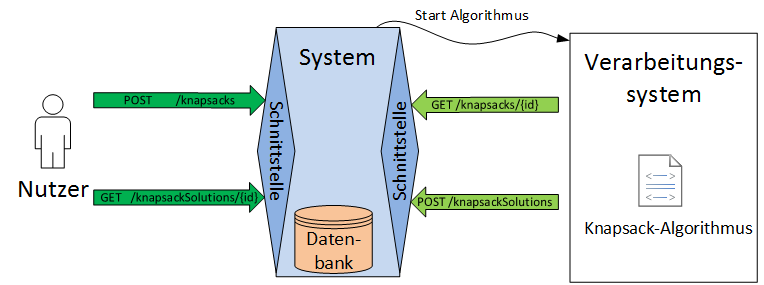
\includegraphics[scale=0.8]{images/visio/prototype_knapsack.png}
\caption[Vertikaler Durchstich mit dem Rucksack Problem]{Vertikaler Durchstich mit dem Rucksack Problem \selfmade{}}
\label{fig:architektur}
\end{figure}

\subsection{Erkenntnisse nach dem ersten Durchstich}\label{entwicklungsumgebung}
Die Kontaktschnittstelle nach Aussen generisch zu halten, macht aus Gründen der Benutzerfreundlichkeit keinen Sinn. Für den Kunden ist es transparenter, wenn er eine Schnittstelle aufruft, 
welche zum Beispiel 'timetabelSchedule' heisst, als eine generische Schnittstelle, welche 'solveProblem' heisst. Zudem ist nicht möglich nur aus den Daten herauszufinden, was für ein Problem 
gelöst werden möchte und es würde die Validierung der Eingabeparameter erschweren.\\

Das Konzept mit den beiden Translators bietet sehr viel Möglichkeiten und Flexibilität. Es entkoppelt die Nutzer-Schnittstelle komplett von der Schnittstelle für die Algorithmen. Um diese 
Flexibilität ausnutzen zu können, müssen jedoch auch verschiedene Entities für die Nutzer- und Algorithmus-Sicht erstellt werden.\\

In der Business Logik kann viel generisch gehalten werden. Die Repositories, Services und die Interfaces können generisch programmiert werden und bleiben für alle Probleme gleich. Beim 
Controller kann die Logik in einer abstrakten Klasse definiert werden und somit müssen nur noch die Namen der Schnittstellen in der spezifischen Implementation definiert werden. Es zeigte sich, 
dass sich das Konzept bewährt und die weiteren Probleme dementsprechend angepackt werden können.

\section{Implementierung der Probleme}\label{impl_backend}
In diesem Unterkapitel wird für jedes Problem kurz erklärt was beim Prototyp implementiert wurde. Eine ausführliche Schnisstellen Dokumentation ist in \autoref{api_doc} zu finden. Zusätzlich 
wurde noch eine elektronische Dokumentation der Schnisstelle mit Hilfe von Swagger UI erstellt, diese stellt die angebotenen Schnistellen und die Eingabeparemter und Resultat sehr 
übersichtlich dar. Beim Evaluieren des Stundenplan Problems wurde bemerkt, dass es sehr viele verschiedene Planungsprobleme gibt und deshalb wurde ein zusätzlich Planungsproblem gewählt, 
um zu schauen, wie sich die Schnittstelle beisehr ähnlichen Problemen verhält.

\todo{Swagger Bild}

%%%%%%%%%%%%%%%%%%%%%%%%%%%%%%%
%
%
%		Rucksack
%
%
%%%%%%%%%%%%%%%%%%%%%%%%%%%%%%%

\subsection{Rucksack}
Das Rucksack Problem ist aus Sicht der Schnittstelle ein relativ einfaches Problem. Der Nutzer kann aus Benutzerfreundlichkeit bei den Elementen eine Anzahl definieren und muss sie so nicht 
doppelt angeben. Der Algorithmus bekommt eine Liste mit allen Elementen, es gibt nur noch einzelne Elemente und der Name wird nicht weiter gegeben, da er vom Algorithmus nicht benötigt wird. 
Der Algorithmus als Resultat eine Liste von Boolean-Werten zurück, diese müssen zuerst wieder auf die eigentlichen Elemente abgebildet werden. Bei der Validierung wird überprüft, ob die 
Gewichtsschranke nicht überschritten wurde und ob ein Element nicht zu oft verwendet wurde. Letzeres ist zwar bei dem Test-Algorithmus nicht möglich, aber könnte bei einer anderen
Implementation eventuell der Fall sein. Der Benutzer erhält als Resultat eine Liste mit allen Objekten, welche verwendet wurden. Wenn das Objekt mehrmals verwendet wurde, wird die 
entsprechende Anzahl angegeben.

%%%%%%%%%%%%%%%%%%%%%%%%%%%%%%%
%
%
%		Knotenfärbung
%
%
%%%%%%%%%%%%%%%%%%%%%%%%%%%%%%%

\subsection{Knotenfärbung}
Beim Knotenfärbung geht es darum Kollisionen zu vermeiden, dies wurde versucht für den Nutzer möglichst transparent anzubieten. Der Nutzer kann mögliche Werte (z.B. Farben oder 
Frequenzen) angeben, welche die Element zugeteilt bekommen sollen. Der Algorithmus erhält eine Liste mit allen Elementen und ihren Nachbaren. Der Name der Elemente und die möglichen 
Werte werden nicht weiter gegeben. Es wird davon ausgegangen, dass der Algorithmus eine Liste von den Elementen mit den zugewiesenen Werten zurückgibt. Beim Übersetzten werden, falls 
vorhanden, die Werte vom Algorithmus mit den möglichen Werten aus der Benutzereingabe ausgetauscht. Bei der Validierung wird überprüft, ob kein Element den gleichen Wert, wie einer 
seiner Nachbaren hat. Als Resultat erhält der Benutzer eine Liste mit allen Elementen und ihren zugewiesenen Werten.

%%%%%%%%%%%%%%%%%%%%%%%%%%%%%%%
%
%
%		Problem des Handlungsreisenden
%
%
%%%%%%%%%%%%%%%%%%%%%%%%%%%%%%%

\subsection{Problem des Handlungsreisenden}
Der Service bietet nicht nur die kürzeste Route für eine Liste von Wegpunkten an, es ist auch möglich für jeden Wegpunkt eine gewünschte Ankunftszeit und Aufenthaltszeit anzugeben. Der 
Nutzer kann eine Liste von Wegpunkten mit gewünschter Ankunftszeit und Aufenthaltszeit angeben. Der Algorithmus erhält eine Liste mit allen Wegpunkten, bei diesem Schritt wird nichts 
übersetzt. Es wäre jedoch möglich, dass die Schnittstelle bereits die Distanzen zwischen den Wegpunkten berechnet oder die Daten sonst irgendwie für den Algorithmus aufbereitet. Es wird 
davon ausgegangen, dass der Algorithmus eine Liste von den Wegpunkten in der berechneten Reihenfolge zurückgibt. Beim Übersetzten werden die geplanten Ankunftszeiten berechnet, 
welche dann während der Validierung mittels der maximal angegebenen Abweichung überprüft werden. Der Benutzer erhält als Resultat eine Liste mit der berechneten Reihenfolge der 
Wegpunkte und jeder Wegpunkt besitz die gewünschte und die geplante Ankunftszeit.

%%%%%%%%%%%%%%%%%%%%%%%%%%%%%%%
%
%
%		Briefträgerproblem
%
%
%%%%%%%%%%%%%%%%%%%%%%%%%%%%%%%

\subsection{Briefträgerproblem}
Das Briefträgerproblem berechnet eine Route, welche alle bekannten Wege einer Strecke abfährt. Der Nutzer kann eine Liste von Wegpunkten mit den bekannten Verknüpfungen zu anderen 
Wegpunkten und ihrer Dinstanz angeben. Der Algorithmus erhält eine Liste mit allen Wegpunkten, die Namen der Wegpunkte werden nicht weitergegeben. Es wird davon ausgegangen, dass 
der Algorithmus eine Liste von den Wegpunkten in der berechneten Reihenfolge zurückgibt. Beim Übersetzten werden die Wegpunkte wieder auf die Eingabewerte abgebildet und die komplette 
Länge der Route berechnet. Die Validierung überprüft, ob der Weg möglich ist und ob jede Verbindung ein Mal benutzt wurde. Der Benutzer erhält als Resultat eine Liste mit der berechneten 
Reihenfolge der Wegpunkte und die totale Länge der Strecke.

%%%%%%%%%%%%%%%%%%%%%%%%%%%%%%%
%
%
%		Stundenplan Design
%
%
%%%%%%%%%%%%%%%%%%%%%%%%%%%%%%%

\subsection{Stundenplan Design}
Die Erstellen eines Stundenplans ist ein Planungsproblem mit sehr vielen Möglichkeiten Einschränkungen zu definieren und somit sehr komplex. In dieser Implementation sind noch bei weiten 
nicht alle Spezialitäten abgedeckt. Es wurde jedoch geschaut, dass bereits einige Einschränkungen, wie zum Beispiel freie Tage von Lehrern und blockierte Schulzimmer, miteinbezogen werden. 
Der Nutzer gibt eine Liste von Klassen, Lehrern, Schulzimmern und Schulfächern an. Die Klassen haben eine Grösse und definieren auch welche Fächer sie besuchen müssen. Die Lehrer haben 
eine Liste mit Schulfächern, welche sie unterrichten können, eine List mit zugehörigen Klassen und eine Definition ihrer freien Tage. Die Klassenzimmer besitzen eine Liste mit möglichen 
Schulfächern und eine Sperrlist, in welcher definiert ist, wann der Raum nicht verfügbar ist. Die Schulfächer können definieren, ob sie eine Raum brauchen, welcher expliziet dafür 
bestimmt ist, zum Beispiel Turnen in der Turnhalle. Neben den Elementen, welche verplant werden, gibt es noch Randbedingungen wie die Pausenzeiten, die Lektionsdauer und die Definition, 
wann unterrichtet werden soll. Der Algorithmus erhält eine Liste mit allen Klassen, Lehrern, Schulzimmern und Schulfächern. Die Rahmenbedingungen werden in Zeitschlitze umgewandelt, 
welche vom Algorithmus verplant werden können. Zusätzlich werden die Elemente etwas generischer benannt, damit der Algorithmus nicht verschiedene Konfigurationen für verschiedene 
Planungsprobleme haben muss. In \autoref{lst:cat_input_timetableScheduling} ist ein Beispiel für eine Eingabe der Rahmenbedingungen gezeigt, welche durch den Translator in die 36 Zahl 
umgewandelt werden würde. Die Zahl wird aus der Lektionsdauer, den Pausen und den einzelnen Zeitfenstern pro Tag berechnet, die \autoref{table:timeslice_calc} stellt dies visuell dar.

\begin{lstlisting}[language=JSON, caption=Ausschnitt einer Eingabe für das Stundenplanproblem für die Rahmenbedingungen, label=lst:cat_input_timetableScheduling]  
{
  ...
  "configuration": {
    "breakTimeSliceSize": [5, 20, 5, 90, 5, 20, 5],
    "dayTimeSlots": [
      {
        "monday": {"defaultTimes": true},
        "tuesday": {"defaultTimes": true},
        "wednesday": {"from": [8, 20, 0], "to": [12,0,0]},
        "thursday": {"defaultTimes": true},
        "friday": {"defaultTimes": true}
      }
    ],
    "lessonDuration": 45
  }
}
\end{lstlisting}

\begin{table}[ht]
\centering
  \begin{tabular}{ l | c | c | c | c | c }
	\hline
	\rowcolor{gray}
	\textbf{Uhrzeit} 	& \textbf{Mo}	& \textbf{Di} 	& \textbf{Mi}	&  \textbf{Do}	&  \textbf{Fr}\\ \hline
	0820-0905		& 1			& 9			& 17			& 21			& 29		\\ \hline
	0910-0955		& 2			& 10			& 18			& 22			& 30		\\ \hline
	1015-1100		& 3			& 11			& 19			& 23			& 31		\\ \hline
	1105-1150		& 4			& 12			& 20			& 24			& 32		\\ \hline \hline
	1320-1405		& 5			& 13			& -			& 25			& 33		\\ \hline
	1410-1455		& 6			& 14			& -			& 26			& 34		\\ \hline
	1515-1600		& 7			& 15			& -			& 27			& 35		\\ \hline
	1605-1650		& 8			& 16			& -			& 28			& 36		\\ \hline
  \end{tabular}
   \caption{Visuelle Darstellung der Zeitfenster Berechnung}\label{table:timeslice_calc}
\end{table}

\FloatBarrier

Es wird davon ausgegangen, dass der Algorithmus eine Liste von Planungskombinationen zurück gibt. Eine Kombination besteht aus einer Zeitfensternummer, einem Lehrer, einer Klasse, 
einem Schulfach und einem Klassenzimmer. Beim Übersetzten werden die IDs auf die ursprünglichen Elemente abgebildet und die Zeitfensternummern werden in Uhrzeiten umgewandelt. 
Zusätzlich wird eine Statistik für die Lehrer geführt, wie viele Stunden sie einzelne Fächer unterrichten. Bei der Validierung wird geschaut, ob ein Element zu einer Zeit zwei Mal verplant ist, 
ob der Lehrer die nötigen Fähigkeiten hat und ob ein Klassenzimmer für das Fach ausgelegt ist. Das Resultat für den Nutzer enthält eine Liste mit den berechneten Kombination, sortiert nach 
Wochentag und Uhrzeit. Die Lehrerstatistik zeigt, wie oft ein Lehrer ein bestimmtes Fach unterrichtet und wie viel Stunden er insgesamt unterrichtet.

%%%%%%%%%%%%%%%%%%%%%%%%%%%%%%%
%
%
%		Spielplan Design
%
%
%%%%%%%%%%%%%%%%%%%%%%%%%%%%%%%

\subsection{Spielplan Design}
Eine weitere Ausprägung des Planungsproblem ist das Erstellen eines Spielplans.Der Nutzer gibt eine Liste von Teams, Schiedsrichter, Spielfelder und Kategorien an. Die Teams haben eine 
bestimmte Kategorie. Die Schiedsrichter haben eine Liste mit Kategorien, welche sie pfeiffen können. Die Spielfelder besitzen eine Liste mit möglichen Kategorien. Neben den Elementen, welche 
verplant werden, gibt es noch Randbedingungen wie die Spieldauer, der Startpunkt und die Pausenzeiten. Der Algorithmus erhält eine Liste mit allen Teams, Schiedsrichter, Spielfelder und 
Kategorien. Zusätzlich werden die Elemente etwas generischer benannt, damit der Algorithmus nicht verschiedene Konfigurationen für verschiedene Planungsprobleme haben muss.

Es wird davon ausgegangen, dass der Algorithmus eine Liste von Planungskombinationen zurück gibt. Eine Kombination besteht aus einer Zeitfensternummer, einem Schiedsrichter, 
einer Kombination von zwei Teams und einem Spielfeld. Beim Übersetzten werden die IDs auf die ursprünglichen Elemente abgebildet und die Zeitfensternummern werden in Uhrzeiten 
umgewandelt. Zusätzlich wird eine Statistik für die Schiedsrichter und die Teams geführt, wie viele Einsätze sie jeweils haben. Bei der Validierung wird geschaut, ob ein Element zu einer Zeit zwei 
Mal verplant ist, ob die Schiedsrichter die nötigen Fähigkeiten haben und ob ein Spielfeld für die Kategorie ausgelegt ist. Der Benutzer erhält als Resultat eine Liste mit den berechneten 
Kombination, sortiert nach Uhrzeit. Die Schiedsrichterstatistik zeigt, wie oft ein Schiedsrichter eine bestimmte Kategorie pfeifft und für wie viel Spiele er insgesamt verantwortlich ist. Die 
Teamstatistik zeigt, wie viele Spiele eine Kategorie insgesamt hat und wie viele Spiele ein Team bestreitet. In \autoref{lst:cat_result_matchScheduling} wird eine Ausschnitt der 
Schiedsrichterstatistik dargestellt.

\begin{lstlisting}[language=JSON, caption=Ausschnitt eines Resultats einer Spielplan Erstellung, label=lst:cat_result_matchScheduling]  
{
  ...
  name: "Sabine Pfister"
  statisticMap: {
    Knaben: 1
    Damen Kat A: 3
    Damen Kat B: 2
    _TOTAL: 6
  }
  ...
}
\end{lstlisting}

\subsection{Übersicht der Schnittstellen}
Die Schnittstellen wurden für die Nutzer- und Algorithmus-Sicht unterschiedlich benannt, um die Verknüpfung nicht zu verlieren und eine Übersicht über alle angebotenen Schnittstellen zu haben,
wurde sie in der \autoref{table:overview_api_interfaces} zusammengetragen.

\begin{table}[ht]
\centering
  \begin{tabular}{ l | l }
	\hline
	\rowcolor{gray}
	\textbf{Nutzer}							& \textbf{Algorithmus}					\\ \hline
	/									& /algorithm/							\\ \hline
	\multicolumn{2}{|c|}{\textbf{Rucksack}}\\ \hline
	 POST /optimalPackComputations					& GET /knapsackComputations/<ID>			\\ \hline
	GET /optimalPackComputations/<ID>/solutions		& POST /knapsackComputations/<ID>/solutions	\\ \hline
	\multicolumn{2}{|c|}{\textbf{Knotenfärbung}}\\ \hline
	POST /avoidCollisionComputations				& GET /graphColoringComputations/<ID>		\\ \hline
	GET /avoidCollisionComputations/<ID>/solutions		& POST /graphColoringComputations/<ID>/solutions	\\ \hline
	\multicolumn{2}{|c|}{\textbf{Problem des Handlungsreisenden}}\\ \hline
	POST /shortestRouteComputations				& GET /tspComputations/<ID>				\\ \hline
	GET /shortestRouteComputations/<ID>/solutions		& POST /tspComputations/<ID>/solutions		\\ \hline
	\multicolumn{2}{|c|}{\textbf{Briefträgerproblem}}\\ \hline
	POST /coverAllConnectionComputations				& GET /postmanComputations/<ID>			\\ \hline
	GET /coverAllConnectionComputations/<ID>/solutions 	& POST /postmanComputations/<ID>/solutions	\\ \hline
	\multicolumn{2}{|c|}{\textbf{Stundenplan Design}}\\ \hline
	POST /timetableScheduleComputations				& GET /timetableScheduleComputations/<ID>			\\ \hline
	GET /timetableScheduleComputations/<ID>/solutions	& POST /timetableScheduleComputations/<ID>/solutions	\\ \hline
	\multicolumn{2}{|c|}{\textbf{Spielplan Design}}\\ \hline
	POST /matchesScheduleComputations				& GET /matchesScheduleComputations/<ID>			\\ \hline
	GET /matchesScheduleComputations/<ID>/solutions		& POST/matchesScheduleComputations/<ID>/solutions	\\ \hline
  \end{tabular}
   \caption{Übersicht der angebotenen Schnittstellen}\label{table:overview_api_interfaces}
\end{table}

\FloatBarrier

\subsection{Erstellung eines neuen Problems}
Um die Schnittstelle um ein neues Problem zu erweitern, muss folgendes gemacht werden...


\FloatBarrier

\subsection{Technische Umsetzung und Probleme}
Das Fundament der Software war mit Spring-Boot \cite{spring_boot} sehr schnell gebaut, die Anbindung an die MongoDB wurde mit SpringData \cite{spring_data} realisiert. Leider waren 
oftmals die Dokumentationen nicht ausreichen oder nur für die XML-Konfiguration von Spring. Weiter gab es fehlende Teile in SpringData, welche mühesam herausgefunden werden mussten. 
So gibt es zum Beispiel zu diesem Zeitpunkt standardmässig keine Möglichkeit ein 'LocalTime'-Objekt oder ein 'LocalDateTime'-Objekt von Java8 zu persistieren. Dies führte zu einem 
Stackoverflow anstatt einem Fehler, was wiederum die Suche nach dem Fehler erheblich erschwerte. Um diese Probleme zu beheben, musste ein eigener Converter geschrieben und dieser 
dann bei der MongoDB Konfiguration angegeben werden.

\newpage

\section{Entwicklungsumgebung}\label{entwicklungsumgebung}
Ein Softwareprojekt benötigt immer eine gewisse Entwicklungsumgebung. Bei der Entwicklung mit Spring-Boot sind die Anfoderungen minimal, da Spring-Boot bereits einen eigenen Webserver 
mitbring.

\subsection{IDE - Integrated Development Environment}
Als \glossarmark{IDE} wurde IntelliJ verwendet, IntelliJ bietet gut Refactoring-Methoden an und ist eine grosse Unterstützung beim Programmieren von Java-Code. Die \glossarmark{IDE} 
bietet auch die Möglichkeit Klassen-Diagramme zu erstellt und hat ein \glossarmark{VIM}-Plugin mit dem bekannte \glossarmark{VIM}-Befehle benutzt werden könne, was die 
Geschwindigkeit beim Programmieren enorm erhöht.

\begin{figure}[h]
\centering
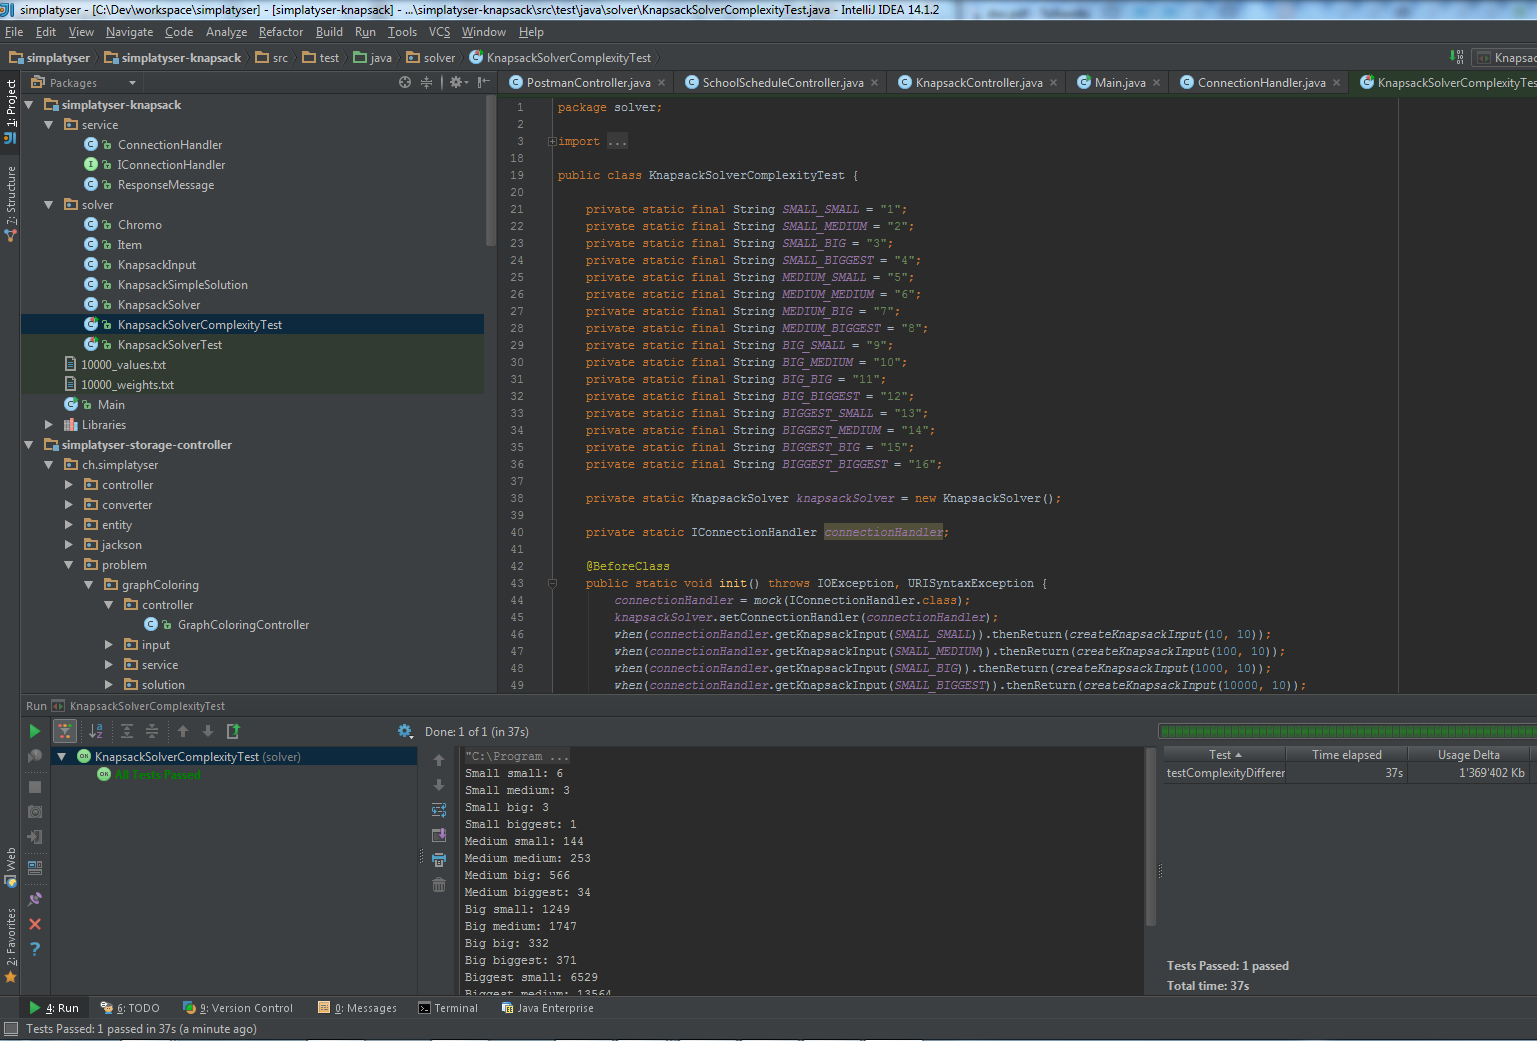
\includegraphics[scale=0.4]{images/intellij.png}
\caption[Test Ausführung in Intellij]{Test Ausführung in Intellij \selfmade{}}
\label{fig:intellij}
\end{figure}

\subsection{Versionierung}
Für die Versionierung der Software wurde git (siehe \cite{git}) verwendet. Das Remote Repository wurde auf Github (siehe \cite{github_simplatyzer}) erstellt. Es wurde darauf geachtet, dass 
der Code oft ins Repository geladen wurde, damit ein Backup existiert. Die Dokumentation wurde in Dropbox gespeichert, damit auf verschiedene Computer darauf zu gegriffen werden konnte 
und immer ein Backup vorhanden ist. Zu Korrekturzwecken wurde die Arbeit dann ebenfalls auf github hochgeladen und die Änderungen konnten dann mit Latexdiff verglichen werden.

\begin{figure}[h]
\centering
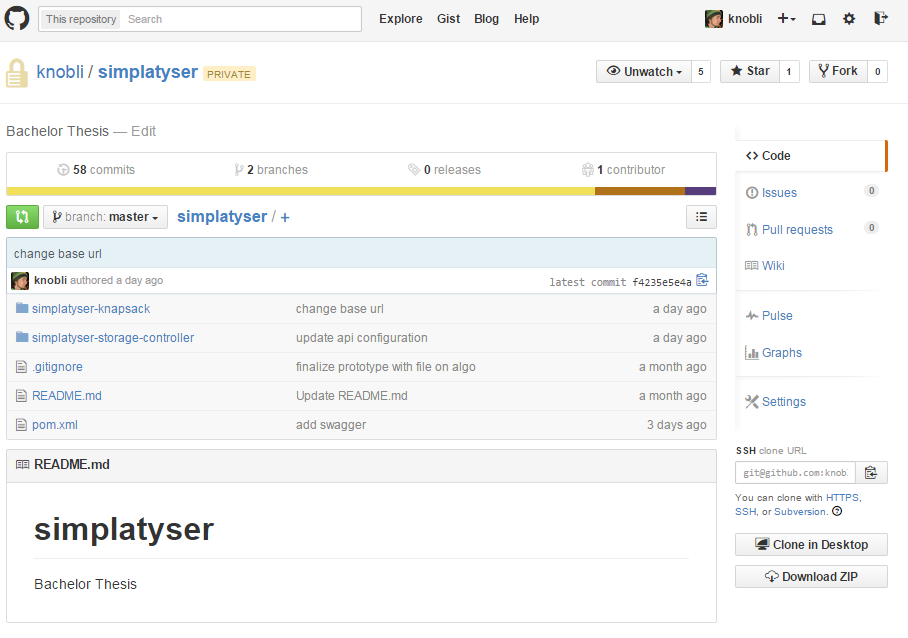
\includegraphics[scale=0.5]{images/github.png}
\caption[Github Repository des Simplatyser Projekts]{Github Repository des Simplatyser Projekts \selfmade{}}
\label{fig:github_repo}
\end{figure}

\subsection{Testen - Analysieren}
 Über den Chrome App 'Advanced REST client' (siehe Abbildung \ref{fig:advanced_rest_client})  wurde die Schnittstelle manuell getestet. Für die Regretion-Tests wurde Junit und Mockito 
verwendet. Die statische Code Analyse wurde mit \glossarmark{Sonar} \cite{sonar} durchgeführt.

\begin{figure}[h]
\centering
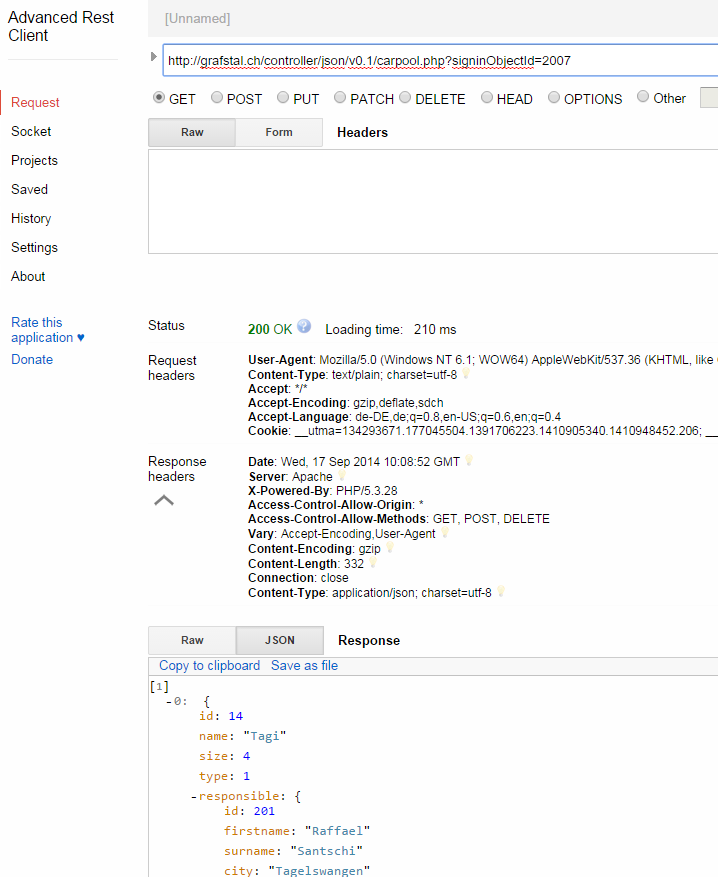
\includegraphics[scale=0.7]{images/advanced_rest_client.png}
\caption[Advanced Rest client]{Advanced Rest client \selfmade{}}
\label{fig:advanced_rest_client}
\end{figure}